\chapter{Purpose and Overview of the Framework}

\subsubsection{Purpose}

The developed Android Framework for accessing USB mass storage devices shall meet determinate requirements:

\begin{itemize}
\item The mass storage device is accessible without root rights
\item The API provides methods for enumerating through all connected mass storage devices and their partitions
\item The API is easy to use and orientates towards the java.io.File API
\item The Frameworks provides basic features like: Adding and removing directories/files, read and write access to files, moving directories/files located on the same volume
\item The Framework shall be licensed under the Apache License, Version 2\footnote{\url{http://www.apache.org/licenses/LICENSE-2.0.html}}
\end{itemize}

The Framework shall at least support the bulk only transfer mass storage devices, which are using the SCSI transparent command set. It shall support devices which are formatted with the MBR partition table and the FAT32 file system. Despite the framework a simple example application shall also be developed to test and demonstrate the framework. The framework and the example application are publicly available at github\footnote{\url{https://github.com/mjdev/libaums}}.

The following parts will describe the framework and the example application, but not every part of the source code is described in detail. If you want to get an insight how the hole things work, you should look into the source code directly, which is also documented.

\subsubsection{Overview}
\label{implementation_overview}

This sections gives a short overview over the hole framework, in the following chapter important parts of the framework will then discussed in detail.

The framework and the example application are purely developed in Java because that is Android's main language for developing applications. The framework uses the standard Java API and the Android USB host API to access USB devices. The example application uses the API of the developed framework and the standard Android API for creating user interfaces.

The framework can roughly be structured in three parts, Figure \ref{figure:package} shows a UML package diagram of the framework. The packages in the UML diagram correspond to the Java packages in the source code. Please note that the UML diagrams in this thesis are often simplified and are not always exactly correct.

\begin{figure}[h!]
\caption{Package overview of the framework.}
\centering
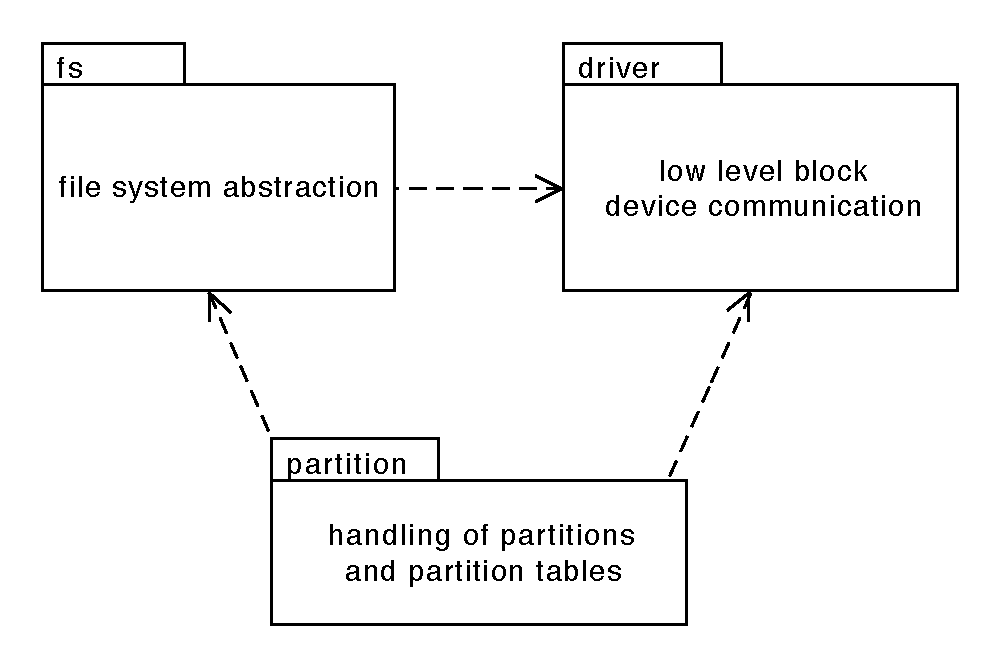
\includegraphics[scale=0.9]{figures/package}
\label{figure:package}
\end{figure}

\subsubsection{Driver}

The driver package is responsible for the low level communication with the block device over USB. It uses USB bulk transfers to access the and communicate with the USB device. It contains the SCSI commands described in the theory part. The package provides then methods for reading and writing raw data from and to the device storage.

\subsubsection{Partition}

This package is relevant for handling partition tables and recognizing the different partitions and their file systems on the mass storage device. Thus it needs direct access to the block device, but also access to the file system implementations. The partition package contains code for handling MBR partition tables.

\subsubsection{File system}

The fs package contains the code for the FAT32 file system. It needs direct access to the block devices' raw data, moreover the raw data of the specific partition it represents. That means it only has indirect access to the driver package, all method calls to read or write raw data are routed through the partition package, to handle the different partitions on a block device correctly.

\subsubsection{UsbMassStorageDevice}

The UsbMassStorageDevice class is the main entry point for accessing mass storage devices. It provides a static method which returns all available mass storage devices. This method loops through all connected USB devices and checks if the connected device is a valid device following the USB mass storage class. The mass storage devices can then be initialized, via the init() method. The initialization process consists of reading the partition table, creating the corresponding partitions and evaluating the desired file system for each partition.  The available partitions can then easily be accessed via a getter. The close method closes the USB communication and releases the USB Interface.

\begin{figure}[h!]
\caption{UML class diagram of the UsbMassStorageDevice.}
\centering
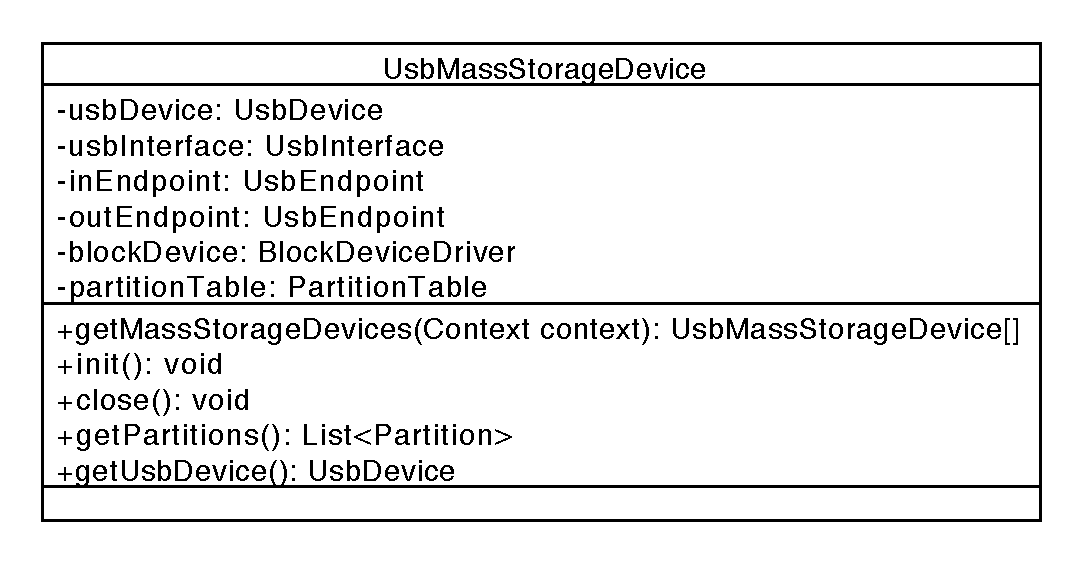
\includegraphics[scale=0.85]{figures/usb_mass_dev}
\label{figure:mass_dev}
\end{figure}

The class also has a lot of private members for communicating with the USB device via the Android API. There is a getter for the underlying UsbDevice, mainly for requesting the permission for communication by the user. Remember the section about the Android USB host API, where requesting a permission is described.

\subsubsection{Partition}

The class Partition represents a single volume on a mass storage device. It provides a getter for the volume label and a getter for the file system to access the contents of the partition.

\subsubsection{FileSystem}

The FileSystem interface also provides a getter for the volume label, which returns exactly the same string like the getter in the class Partition. In fact the getter of the Partition class simply delegates the call to the FileSystem class. The next important method is for accessing the root directory of the file system and listing it contents.

\subsubsection{UsbFile}

The UsbFile interface represents an abstraction for files and directories. Every directory or file is an UsbFile. The root directory returned by the FileSystem interface is also a UsbFile. The UsbFile interface provides various methods to access and modify the contents of a file or directory. For a complete documentation on every method please refer to the javadoc in the source code. Note that some methods only make sense for directory or files, but not both for of them!

\begin{figure}[h!]
\caption{UML class diagram of the UsbFile interface.}
\centering
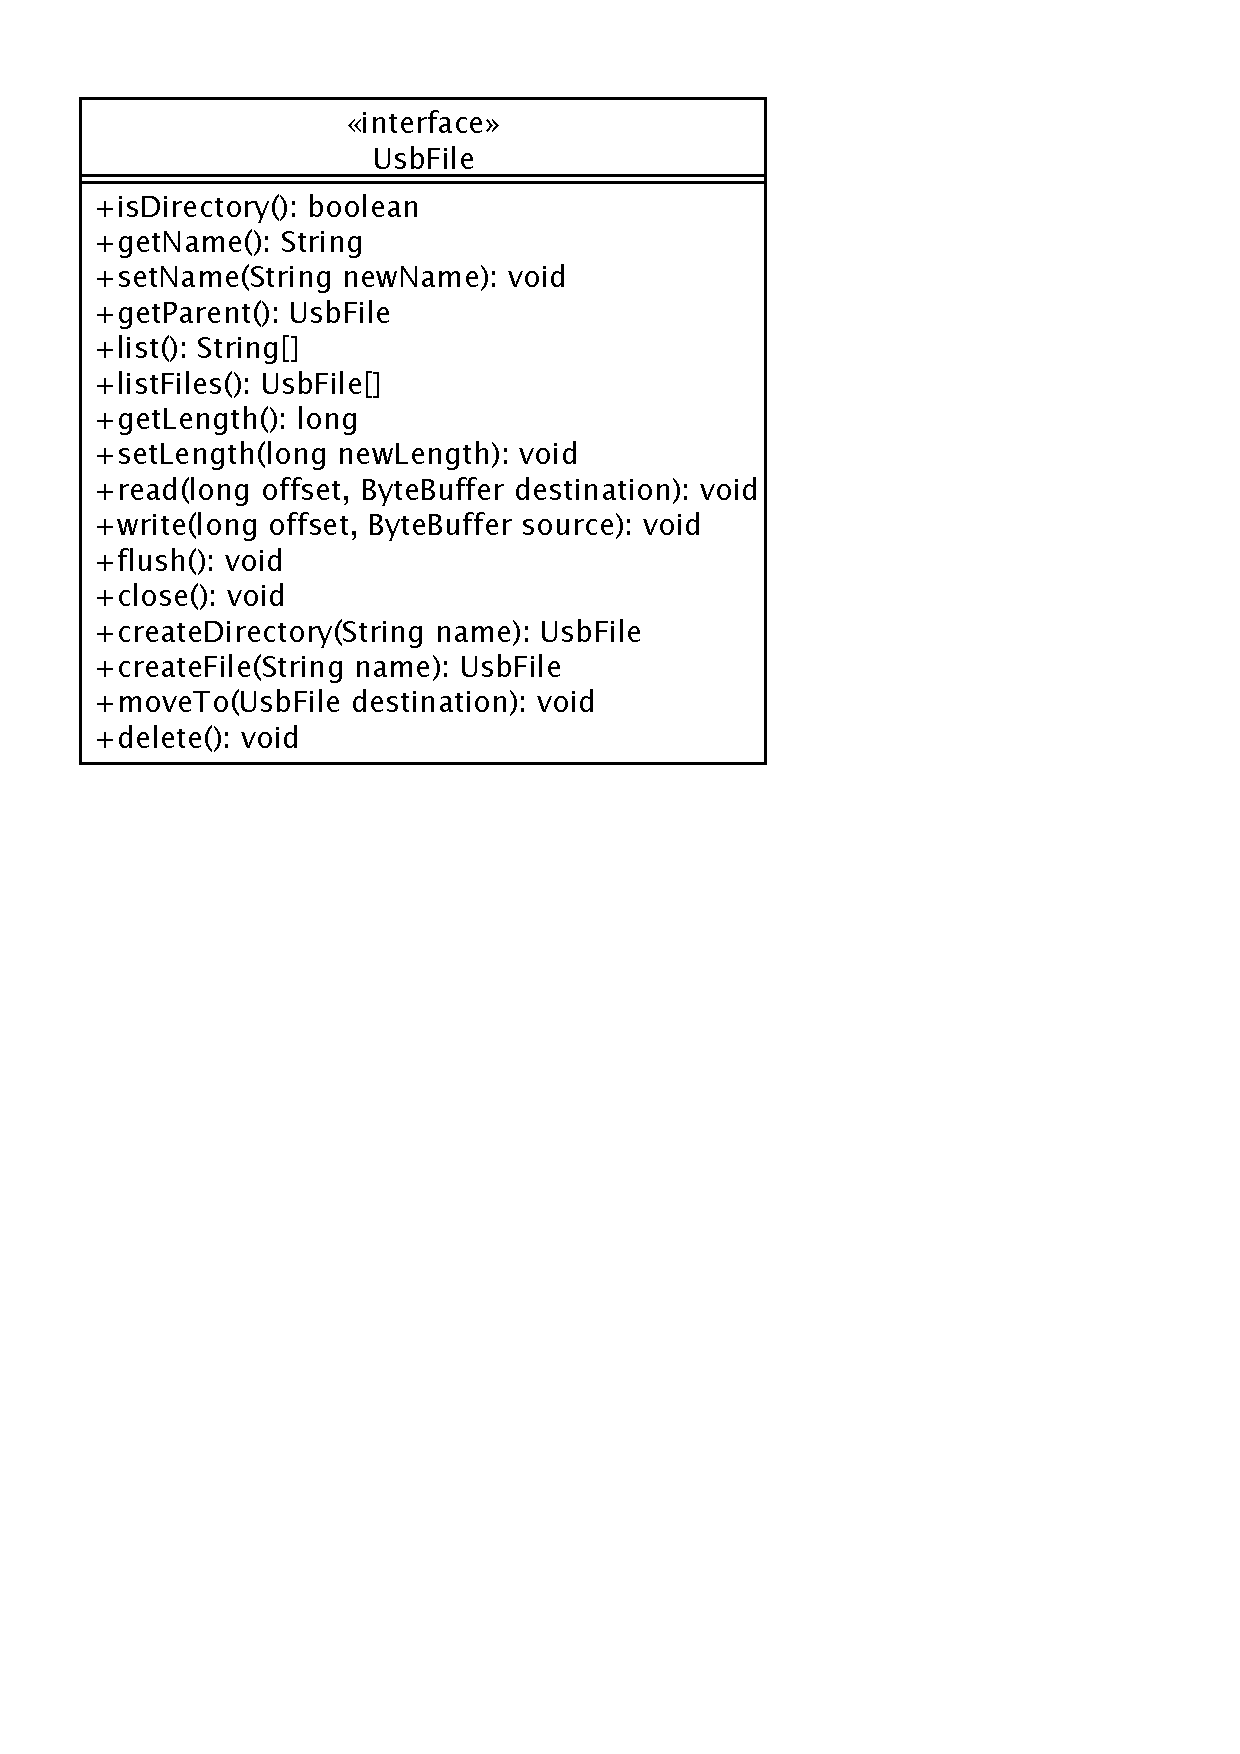
\includegraphics[scale=0.85]{figures/usb_file}
\label{figure:usb_file}
\end{figure}

\subsubsection{Code example}

The following code demonstrates the use of the classes introduced above. The example simply takes the first USB mass storage device which could be found and lists the contents of the root directory of the first partition.

\lstset{language=Java}
\begin{lstlisting}[caption=Code example for accessing the contents of a mass storage device, label=listing:main_example]

private void setupDevice() {
    // the getter needs a Context as a parameter so make sure to call the method
    // in an Activity or Service, etc.
    UsbMassStorageDevice[] devices = UsbMassStorageDevice.getMassStorageDevices(this);
    		
    if(devices.length == 0) {
        Log.w(TAG, "no device found!");
        return;
    }
	
    UsbMassStorageDevice device = devices[0];
	
    try {
        // before initializing the device, make sure the user has granted the permission to communicate
        // this can be done with the UsbManager class and a BroadcastReceiver like shown in the
        // section about the Android USB Host API
        device.init();
		
        // we always use the first partition of the device
        FileSystem fs = device.getPartitions().get(0).getFileSystem();
        Log.d(TAG, "volume label: " + fs.getVolumeLabel());
		
        UsbFile root = fs.getRootDirectory();
        String[] contents = root.list();
        for(String str : contents) {
            Log.d(TAG, str);
        }
    } catch (IOException e) {
        Log.e(TAG, "error setting up device", e);
    }
}
\end{lstlisting}

\chapter{Inside the packages}

\section{The driver package}

As mentioned previously, the driver package is responsible for handling the low level communication with the block device. It can access the USB device via bulk IN and OUT transfers. Currently only a block device driver for the SCSI transparent command set is available.

\begin{figure}[h!]
\caption{UML class diagram of the driver package.}
\centering
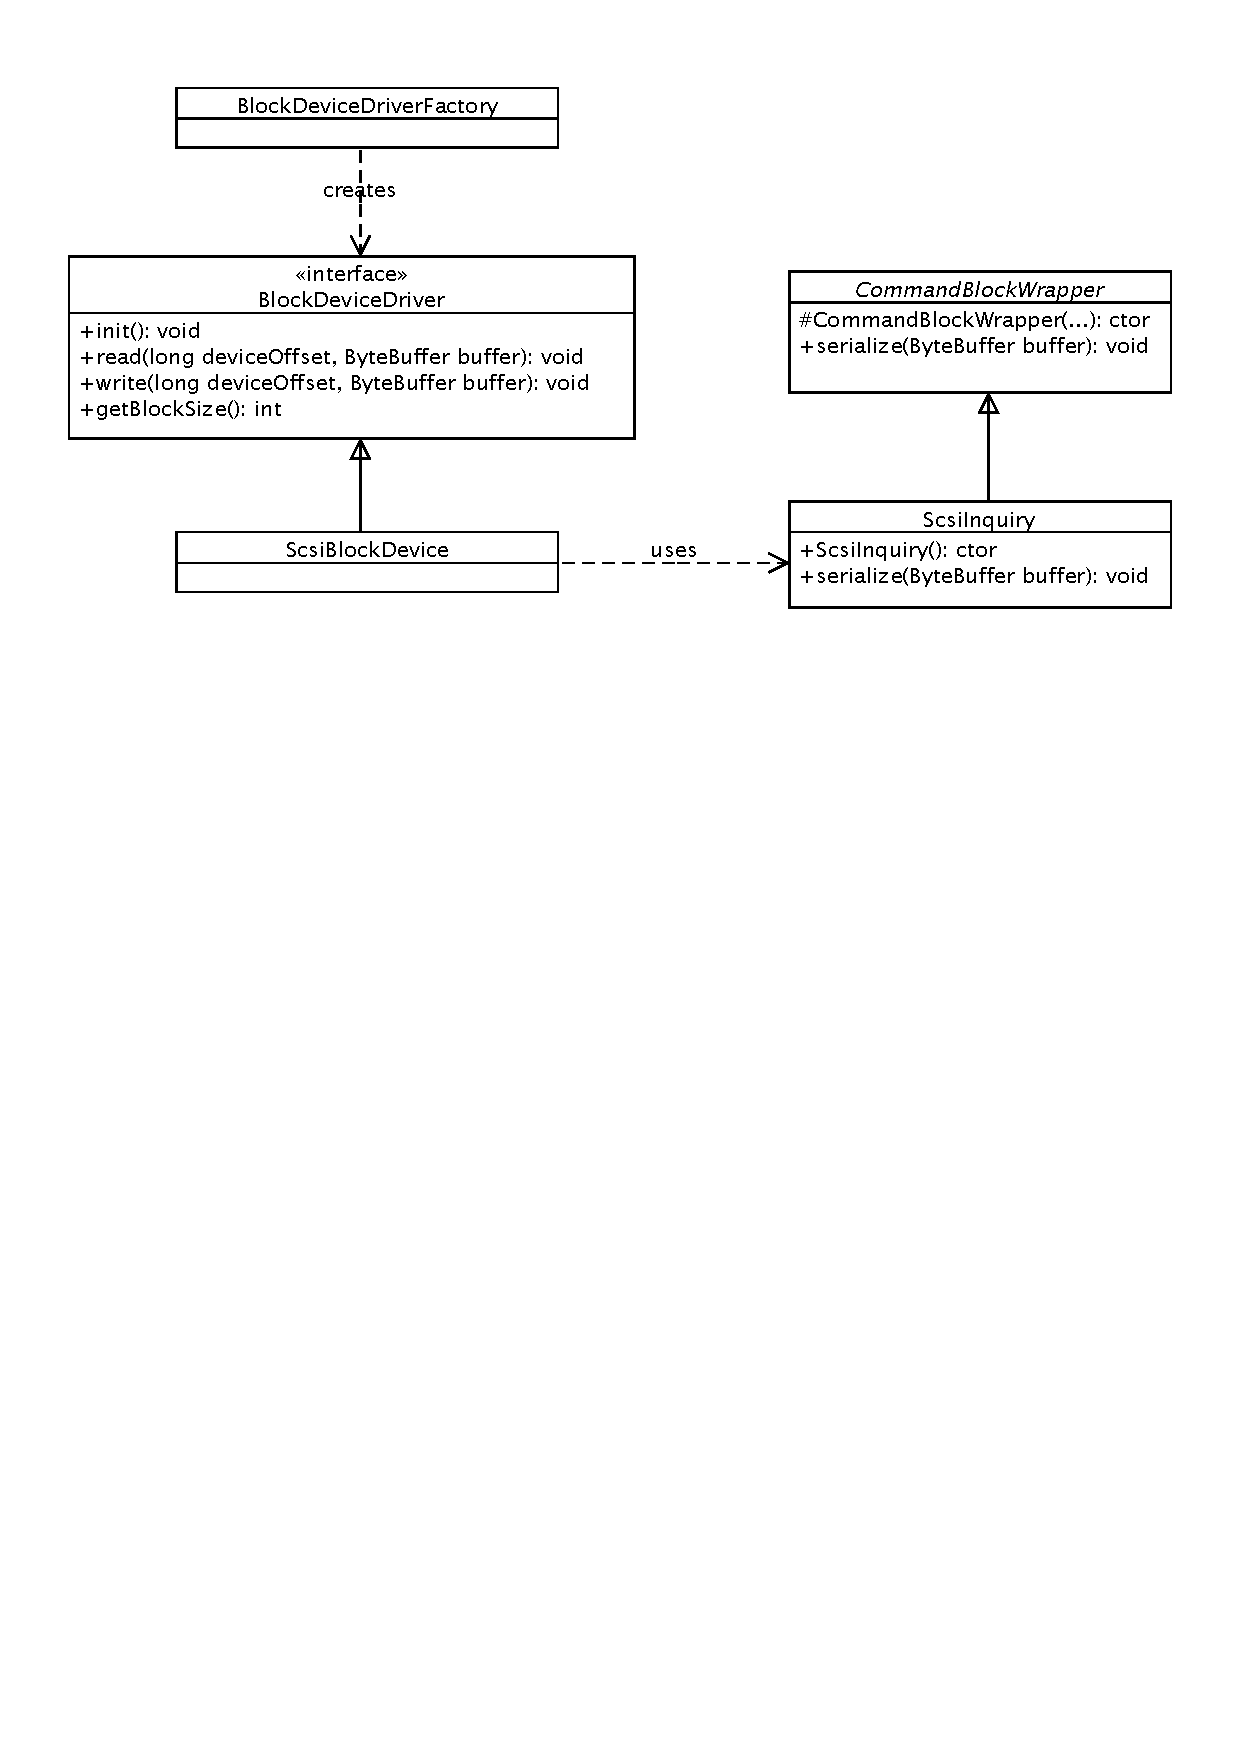
\includegraphics[scale=0.85]{figures/driver_package}
\label{figure:driver_package}
\end{figure}

\subsubsection{BlockDeviceDriver}

The BlockDeviceDriver interface is a general representation of a block device. It provides methods for reading and writing raw data to the devices' media storage. It takes an device offset and a ByteBuffer as parameters to determine the starting offset of a read or write. The ByteBuffer indicates the length of the data which shall be read or written. If data shall be read, the data is read into the ByteBuffer, otherwise the data in the ByteBuffer is written to the device. It also offers a getter to determine the block size the connected device uses.

\subsubsection{BlockDeviceDriverFactory}

This class is in charge to create a suitable block device driver for the connected mass storage device. It currently always creates a ScsiBlockDevice because no other driver is currently supported. This class is intended to make further development and integration of other device drivers easier. There are also factory classes in the two other packages for creating suitable partition tables and file systems.

\subsubsection{ScsiBlockDevice}

This is the representation of a block device driver which uses the SCSI transparent command set for communicating with devices. It transfers SCSI commands to the device, receives the desired responses from the device and interprets them.\\

All SCSI commands a modeled in an own class which extend the CommandBlockWrapper. The CommandBlockWrapper is an abstract class which is coupled with a SCSI command. Remember that every SCSI command is enclosed by a CBW in the SCSI transparent command set protocol. The CBW offers a method to serialize itself to a ByteBuffer. This data can then be directly transmitted to the device. The serialized data include the direction of the command, the transfer length in the transport phase and the length of the SCSI command.

Every SCSI command also offers the serialization to a ByteBuffer, it first calls the serialization method of the CBW class (super class) and then adds serializes the own data to the ByteBuffer. Using this approach it is easy to wrap the CBW around the SCSI commands and new commands are easier to implement. 

In the UML diagram \ref{figure:driver_package} only the SCSI INQUIRY command is shown, but there are, of course, also classes for all other commands presented earlier.

\section{The partition package}

The partition package is responsible for handling the partition table on a USB mass storage device. Currently only the MBR partition table is supported. Determining the partition table can be pretty hard, because there is no hint which type of partition table is stored on the device. That means the data at LBA zero has to be read (normally a partition table starts at the beginning of a volume) and it has to be checked if the data represents a valid partition table. Figure \ref{figure:partition_package} illustrates the contents of the partition package. There is again a factory class for creating suitable partition tables, this class currently always creates the MBR partition table.

\begin{figure}[h!]
\caption{UML class diagram of the partition package.}
\centering
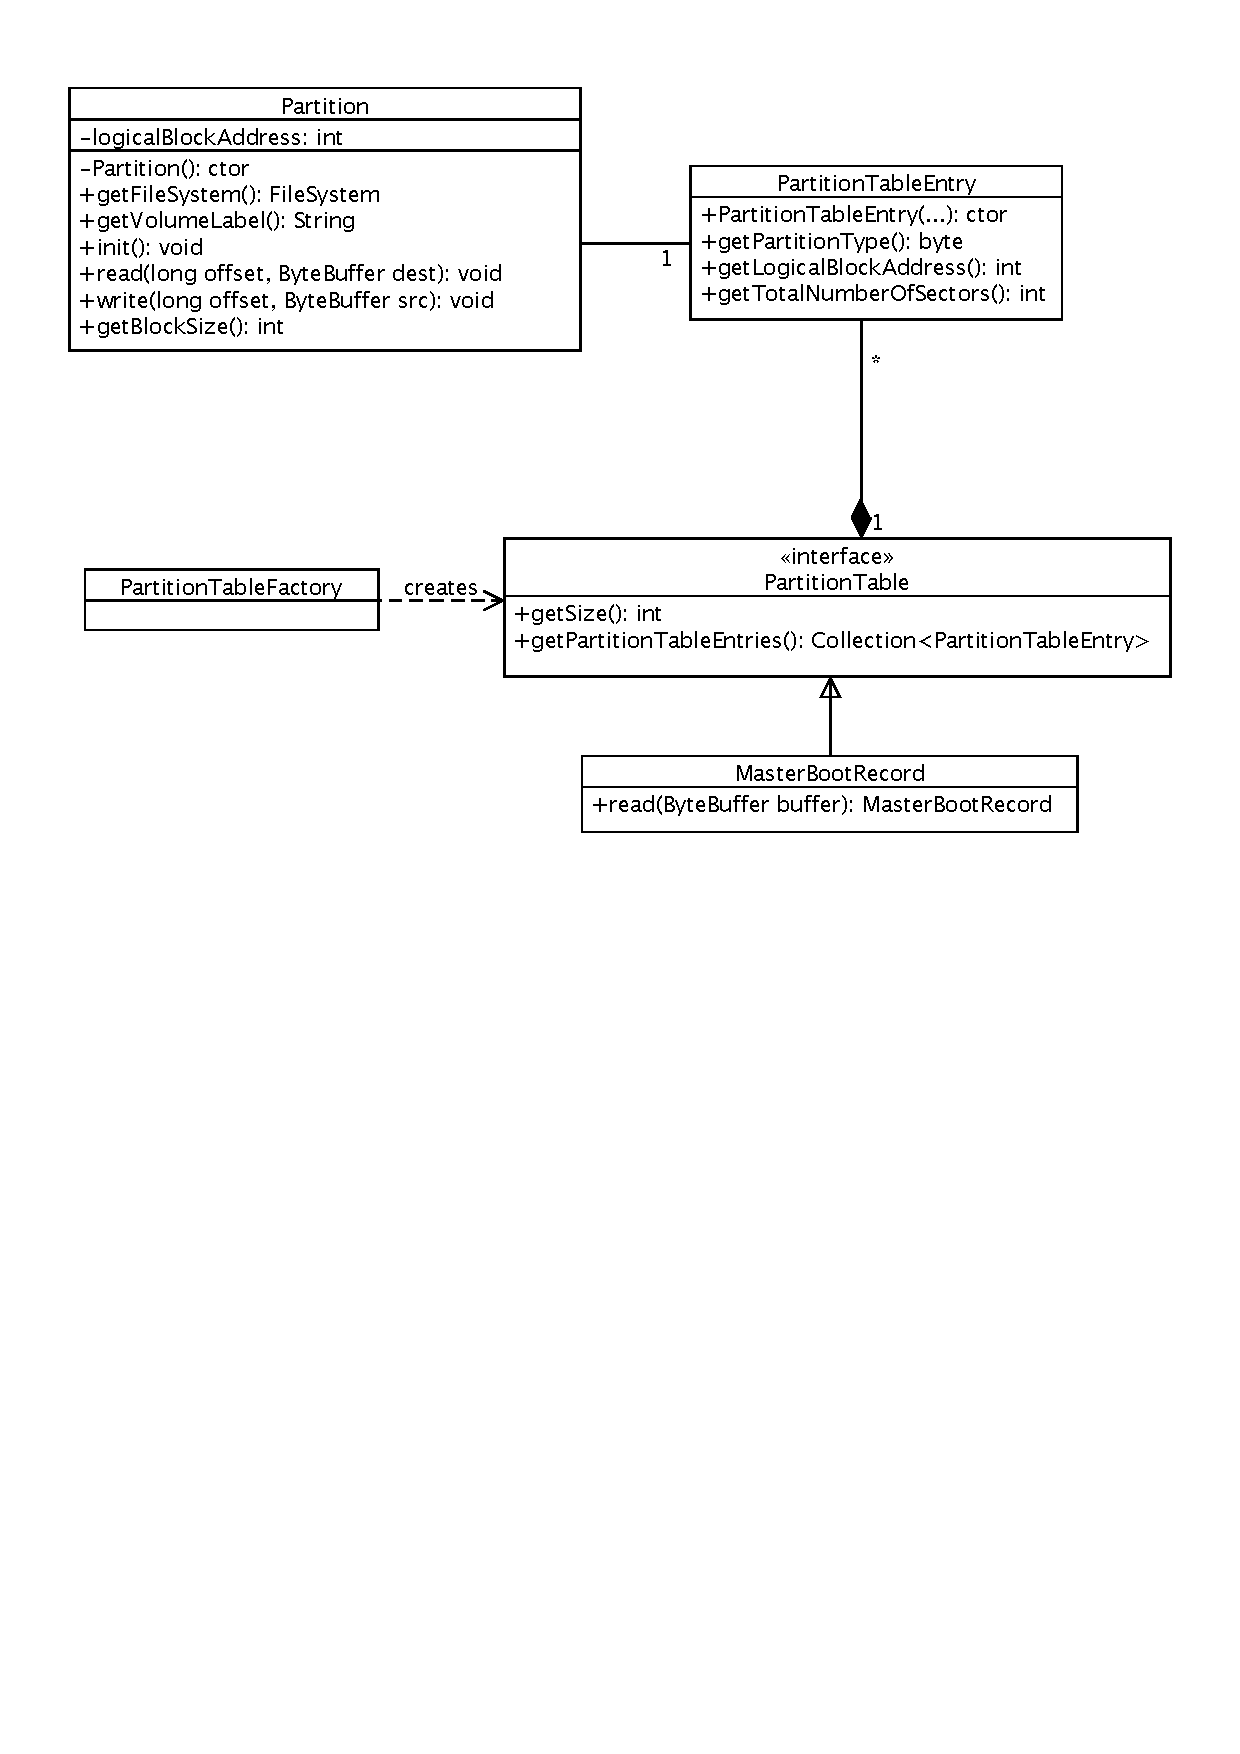
\includegraphics[scale=0.85]{figures/partition_package}
\label{figure:partition_package}
\end{figure}

\subsubsection{PartitionTable}

This interface represents in general a partition table. It provides a getter to receive all partition table entries in the table. There is also a method for getting the size of the partition table. For the MBR this is 512 bytes. The factory class shall use this size, to determine how many bytes from the mass storage device have to be read.

\subsubsection{PartitionTableEntry}

The PartitionTableEntry represents the information of a partition stored in the partition table. It saves the logical block address where the partition starts, the total number of sectors/blocks the partition occupies and the type of the partition. This is mostly the file system type of the partition, but in case of the MBR this could also be an extended partition.

\subsubsection{MasterBootRecord}

This class covers the Master Boot Record implementation. It has a static read method which returns an instance of the MasterBootRecord class, or null if the data in the ByteBuffer does not look like a Master Boot Record.

\subsubsection{Partition}

The Partition class was already introduced in the overview section (\ref{implementation_overview}), but this time we will have a closer look at how it interacts with the other classes of the package and the file system package. 

The Partition class has access to the PartitionTableEntry it represents. It uses the information of stored in th entry to determine the starting point (LBA) of the partition and to initialize a suitable file system, the user can then access. As you may have noticed, the Partition class implements also the BlockDeviceDriver interface from the driver package, described earlier. This is needed because every partition represents an independent volume of the mass storage device. A file system driver should be independent of the location of a partition, hence the partition is responsible for translating the requests of the file system driver according to the starting point, the logical block address of the partition.